%
%    * ----------------------------------------------------------------
%    * "THE BEER-WARE LICENSE" (Revision 42/023):
%    * Ronny Bergmann <mail@rbergmann.info> wrote this file. As long as
%    * you retain this notice you can do whatever you want with this
%    * stuff. If we meet some day and you think this stuff is worth it,
%    * you can buy me a beer or a coffee in return.
%    * ----------------------------------------------------------------
%
%
% Kartei Source Code of the german manual
%
% Last Change: Kartei 1.9, 2012/01/04
%
\documentclass[a4paper,DIV=calc]{scrartcl}
\usepackage[utf8]{inputenc} %UTF8
\usepackage[OT1]{fontenc}
%\usepackage[scaled]{helvet}
\usepackage[ngerman]{babel} % Neue Rechtschreibung
%Menge an Paketen die für vor allem mathematisches und informatisches gut brauchbar ist
\usepackage{graphicx,hyperref}
\usepackage{enumerate,subfigure,listings}
\usepackage{pdfpages,color}
%\usepackage[pdftex,dvipsnames]{xcolor}
%\usepackage[light]{kpfonts}

\lstloadlanguages{TeX}
\lstset{basicstyle={\rmfamily\footnotesize},numbers=left,numberstyle=\tiny\color{maincolor},numbersep=5pt, breaklines=true, captionpos={t},language={},frame=none,numbers=left,tabsize=3, showspaces=false, showtabs=false, columns=fixed}	
\setlength{\parindent}{1em}
\setlength{\parskip}{0em}	
\setlength{\marginparwidth}{3cm}
\colorlet{maincolor}{black!80}

\hypersetup{
   pdftitle={Karteikarten in LaTeX}%
	  ,pdfauthor={Ronny Bergmann}%
	  ,pdfcreator={LaTeX, hyperref, KOMA-Script, TextMate},
   pdfkeywords={Cards, Karteikarten, TeX, Paket, Anleitung, Manual},
   pdfdisplaydoctitle,
   bookmarksnumbered=true,
   bookmarksopen=true,
   bookmarksopenlevel=1,
   plainpages=false,
   bookmarksnumbered,
   pdfborder={0 0 0}
   }

\addtokomafont{sectioning}{\rmfamily}
\setkomafont{descriptionlabel}{\rmfamily\bfseries}
\newcommand{\befehl}[1]{%
\marginpar{\footnotesize\textsf{#1}}%
}

\begin{document}
\title{Karteikarten in \LaTeX\\{\large Version 1.9}}
\author{Ronny Bergmann\\\emph{mail@rbergmann.info}}
\date{\today}
\maketitle
\section{Einleitung}
Karteikarten sind zum Lernen hilfreich, sei es etwa in kleinem Format für Vokabeln oder für umfangreichere Themen, die man auf größeren Karteikarten stichpunktartig notiert. Zusätzlich zum Lernen am Computer, wo die Karteikarten in einem Dokument vorliegen sollten, möchte man Karteikarten wahrscheinlich auch drucken. Dazu werden mehrere Karteikarten auf eine Seite gesetzt, wobei die zweite Seite „trickreich umsortiert“ wird, damit im Duplex-Druck jeweils die passenden Vorder- und Rückseiten aneinander gedruckt werden. Beide Formate basieren auf dem gleiche Inhalt, so dass hier \LaTeX\ hilfreich sein kann, diese beiden Formate zu produzieren.

Zum Ausprobieren genügt es, die Dateien im gleichen Verzeichnis wie die Hauptdatei der Karteikarten zu hinterlegen. Für umfangreichere Arbeiten sollte man die Dateien in einem speziellen Ordner (\lstinline!/texmf-dist/tex/latex/kartei! als Empfehlung) hinterlegen und \lstinline!sudo texhash! in der Konsole aufrufen.

\section{Dokumentoptionen}
Für eine gesamte Kartei \befehl{\textbackslash document-\\class\{kartei\}}, oder auch Ansammlung von Karteikarten lassen sich zunächst die normalen Optionen für einen Artikel selbst angeben, also etwa die Standardschriftgröße. Werden diese nicht angegeben, so wird die Schriftgröße etwa auf \lstinline!10pt! hesetzt. Karteikarten sind stets im Querformat gesetzt.
\subsection{Kartenformat}
\befehl{aXpaper}
Es gibt die folgenden Karteikartenformate
\begin{description}
	\item[a5paper] Karteikarten im DIN-A5-Format $(210$m$\times 148$mm$)$\footnote{Dank an M. Wolf für die Idee}
	\item[a6paper] Im DIN-A6-Karteikarten-Format $(148$mm$\times 105$mm$)$ sind die Ränder ein wenig größer gewählt als bei den anderen beiden Formaten. Dieses Format ist der Standard, wenn nichts angegeben wird für das Format.
%	 \befehl{a7paper}
	\item[a7paper] DIN-A7-Karteikarten $(105$mm$\times 74$mm$)$
%	 \befehl{a8paper}
	\item[a8paper] DIN-A8-Karteikarten $(74$mm$\times 52$mm$)$, ab hier sollte man die Schriftart kleine als 10\,pt setzen
%	 \befehl{a9paper}
	\item[a9paper] DIN-A9-Karteikarten $(52$mm$\times 37$mm$)$\footnote{Dank an H. Fritsch für den Patch}
\end{description}
\subsection{Varianten im Druck}\befehl{print}
\paragraph{Aktivieren der Druckausgabe}
Durch Angabe der Dokumentoption \lstinline!print! werden die Karteikarten auf einem DIN-A4-Blatt angeordnet, um eine einfache Druckversion zu erzeugen. Diese wird randlos erzeugt, exakt so gedruckt erhält man obige Karteikartenmaße, sonst sind die Karten ein wenig verkleinert.

Auf ungeraden Seite werden je 4 (beziehungsweise 8, 16 oder 32) Vorderseiten, auf der darauf"|folgenden geraden Seite die dazugehörigen Karteikartenrückseiten so angeordnet, dass im Duplex-Druck automatisch doppelseitig bedruckte Karteikarten entstehen.

Die Anordnung bei DIN-A6 (4 Karteikarten pro Blatt) bzw. DIN-A8 (16 pro Blatt) werden die Karten im Querformat gesetzt. Somit wird der Duplex-Druck  \emph{über die kurze Seite geklappt}. Für DIN-A7 werden die Karteikarten im Hochformat gesetzt, dies ergibt im Duplex-Druck also eine Anordnung, bei der die Karten \emph{über die lange Seite geklappt} werden.

\paragraph{Variante der Rückseite}
Außerdem lässt sich mit der Option \befehl{flip}\lstinline!flip! die Rückseite der Karteikarte um $180^{\circ}$ drehen, so dass sie im PDF auf dem Kopf steht. Wendet man dann den Duplexdruck an, sind die Rückseiten überkopf auf den Karteikartem, man dreht (beim Lernen) also nicht mehr auf einer vertikalen Achse, sonder über die horizontale.\footnote{Dank an S. Han für die Idee}

\paragraph{Schnittlinien}
Zum Ausschneiden lassen sich Schnittlinien aktivieren. Dies geschieht durch \befehl{grid=X} \lstinline!grid=X!, wobei \lstinline!X! einer der folgenden 4 Werte ist:
\begin{description}
	\item[none] zeigt keine Schnittlinien
	\item[rear] erzeugt nur auf den Rückseiten die Schnittlinien
	\item[front] analog nur auf der Vorderseite
	\item[both] Schnittlinien auf Vorder- und Rückseite der Karten	
\end{description}
Die Linien, entlang derer geschnitten werden kann, sind auf der Rückseite mit gestrichelten schwarzen, auf der Vorderseite mit ebenso gestrichelten, aber grauen Linien dargestellt. Da sie in \emph{TikZ} realisiert sind, lassen sich diese Angaben auch durch Ändern der entsprechenden Stile anpassen. Die beiden Stile lauten:
\begin{lstlisting}
	\tikzset{front grid/.style={very thin, gray, loosely dashed}}
	\tikzset{rear grid/.style={thin, black, loosely dashed}}
\end{lstlisting}
Die Linienarten lassen sich also variieren, indem man den jeweiligen Stil umdefiniert.
\subsection{Eine Übersicht}
Die Dokumentoption \befehl{toc}\lstinline!toc! erzeugt im Anschluss an die Karteikarten eine Übersicht über alle Karteikarten\footnote{Dank an W. Erdmann für die Idee und hilfreiche Tipps}. Dazu werden die Kartennummern und Titel/Fragen (siehe Abschnitt \ref{def:Karte}) aufgelistet und durch eine Spalte für Notizen ergänzt. In der aktuellen Version (Stand 11. Januar 2011) funktioniert diese Option nur, wenn \lstinline!print! \emph{nicht} gesetzt ist. Andernfalls verhindert \lstinline!pgfpages! noch die Ausgabe.

\subsection{weitere Dokumentoptionen}
Alle weiteren Dokumentoptionen werden nicht direkt von der Karteikartenklasse verarbeitet, sondern an \lstinline!scrartcl! weitergegeben. Dadurch läßt sich per \befehl{Xpt}\lstinline!Xpt! die Schriftgröße verändern, wobei \lstinline!X! ein ganzzahliger Wert sein muss\footnote{Nach einem Vorschlag von C. Schramm}. Weitere Dokumentoptionen der KOMA-Script-Klasse lassen sich auf diesem Wege auch verändern, diese wurden jedoch nicht getestet.

\subsection{Beispiele}
\begin{itemize}
	\item Zum Erstellen von A6-Karteikarten, normal gesetzt \lstinline!\documentclass[a6paper]{kartei}!
	\item Für A7-Karteikarten im Druckformat mit gedrehter Rückseite und Schnittlinien auf beiden Seiten \lstinline!\documentclass[a7paper, print,flip,grid=both]{kartei}!
	\item um etwa die Schriftgröße zu variieren kann die Option der Koma-Script-Klasse genutzt werden \lstinline!\documentclass[a7paper,9pt]{kartei}!.
\end{itemize}
%
%
%
\section{Die Karten}

\subsection{Definition einer Karte}\label{def:Karte}\befehl{\textbackslash begin\{karte\}}

Innerhalb des Dokumentes lassen sich nun einzelne Karteikarten definieren. Dazu gibt es die Umgebung \lstinline!karte!. Karten werden automatisch durchnummeriert und es ist möglich, per \lstinline!\ref{}! auf Karten zu verweisen, die \lstinline!\label{}! enthalten.
Die Umgebung \lstinline!karte! benötigt 3 Parameter, von denen 2 optional sind. Die Parameter und ihre Reihenfolge sind:
\begin{enumerate}[1.]
	\item \textbf{Fach} [optional] Das Fach oder wesentliches Stichwort
	\item \textbf{Titel/Frage} [Pflicht] wesentliche Frage/Titel oder Vokabel der Karteikarte
	\item \textbf{Kommentar} [optional] Ein kurzer Kommentar oder Stichwort, das etwa die Wichtigkeit klassifiziert oder Unterbereiche eines Faches wiedergibt
\end{enumerate}
Innerhalb der Umgebung selbst wird dann die eigentliche Antwort angegeben. Diese wird auf die Rückseite der Karteikarte gesetzt.

\subsection{Layout}
Die Vorderseite enthält im Kopf links das Fach, mittig die Nummer der Karte, rechts den Kommentar. Zentral auf der Vorderseite wird die Frage gesetzt. Auf der Rückseite wird links die Kartennummer wiederholt, mittig der Term „Antwort“.

Die beiden optionalen Werte Fach und Kommentar lassen sich auch global angeben. Eine Angabe bei einer einzelnen Kartei überschreibt allerdings die globale Definition. Die Idee ist dabei, das Fach zu Beginn einmal zu setzen und somit nur bei Ausnahmen eine Einzelangabe bei einer Karte vorzunehmen. Außerdem läßt sich der Antwortterm global neu setzen. Details dazu finden sich im Abschnitt \ref{subsec:Struktur}. Zwei Beispiele für Karteikarten finde sich in den Abbildungen \ref{fig:example} und \ref{fig:completeexample}.
\begin{figure}
\subfigure[][Vorderseite]{\fbox{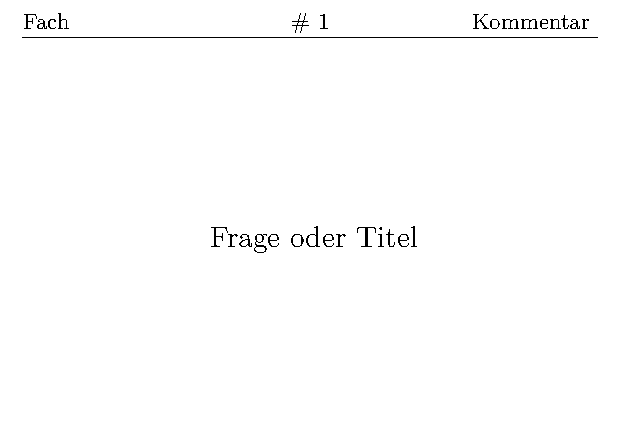
\includegraphics[width=.5\textwidth-2\fboxsep-2\fboxrule,page=1]{manualexample1.pdf}}}
	\quad	\subfigure[][Rückseite]{\fbox{\includegraphics[width=.5\textwidth-2\fboxsep-2\fboxrule,page=2]{manualexample1.pdf}}}
	\caption{Vorder- und Rückseite der exemplarischen Karte in etwas kleiner als DIN-A7}\label{fig:example}
\end{figure}
\begin{figure}
\subfigure[][Vorderseite]{\fbox{\includegraphics[width=.5\textwidth-2\fboxsep-2\fboxrule,page=3]{manualexample1.pdf}}}
	\quad	\subfigure[][Rückseite]{\fbox{\includegraphics[width=.5\textwidth-2\fboxsep-2\fboxrule,page=4]{manualexample1.pdf}}}
	\caption{Vorder- und Rückseite der gefüllten wichtigen Karte, etwas kleiner als DIN-A7}\label{fig:completeexample}
\end{figure}

\subsection{Beispiele}
\paragraph{exemplarisch gefüllte Karteikarte}
Mit den Werten gefüllt, die den Namen der Felder entsprechen, ergibt sich etwa der Code (vgl. Abb. \ref{fig:example})
	\begin{lstlisting}
\begin{karte}[Fach]{Frage oder Titel}[Kommentar]
	Antworttext
\end{karte}
	\end{lstlisting}

\paragraph{Karteikarte mit einer wichtigen Frage}
	Ein wenig mehr gefüllt ist etwa das folgende Beispiel (vgl. Abb. \ref{fig:completeexample}).
	\begin{lstlisting}
\begin{karte}[Lebensphilosophie]
	{Wie lautet die Antwort auf die Frage nach dem Leben dem Universum und dem Ganzen Rest?}
	[wichtig!]
	42
\end{karte}		
	\end{lstlisting}	
%\fach{standardfach}
%\fach{} zum expliziten leeren
%\fachstil{ --stilangabe-- }
%\kommentar{standardfach}
%\kommentar{} zum expliziten leeren
%\kommentarstil{ --stilangabe-- }
%\antwort{Antwort}
%\antwortstil{ --stilangabe-- }

\subsection{Strukturierung}\label{subsec:Struktur}
\paragraph{Fächer \& Kommentare}
Neben der Möglichkeit, bei einer Karte das Fach und den Kommentar explizit anzugeben, lässt sich beides auch global setzen, so dass es bei den darauf"|folgenden Karten verwendet wird und nicht bei jeder Karte einzeln angegeben werden muss.

Mit \lstinline!\fach! (engl. \lstinline!\cardsubject!\befehl{\textbackslash fach\\\textbackslash subject}) gefolgt von einem Text in \lstinline!{geschweiften Klammern}! setzt man das Fach für die nachfolgenden Karten. Die Schriftformatierung kann über Neudefinition des Befehl \lstinline!\fachstil! (engl. \lstinline!\subjectstyle!\befehl{\textbackslash fachstil\\\textbackslash subjectstyle}) vorgenommen werden. Standardmäßig ist der Stil auf \emph{kursiv} gesetzt. Um an einer Stelle den momentanen Wert auszugeben, gibt es den Befehl \lstinline!\dasfach{}! (engl. \lstinline!\thesubject!\befehl{\textbackslash dasfach\\\textbackslash thesubject}). Wird bei einer Karte bei gesetztem Fach trotzdem ein Fach angegeben, so hat das Fach der Karte Vorrang, so kann in einem großen Block auch eine Ausnahmekarte erzeugt werden.

Analog lässt sich der Kommentar global setzen mit \lstinline!\kommentar{Kommentartext}! (engl. \lstinline!\comment!\befehl{\textbackslash kommentar\\\textbackslash comment}), dessen Stil mit \lstinline!\kommentarstil! (engl. \lstinline!\commentstyle!\befehl{\textbackslash kommentarstil\\\textbackslash commentstyle}), respektive die Ausgabe mit \lstinline!\derkommentar! (engl. \lstinline!\thecomment! \befehl{\textbackslash derkommentar\\\textbackslash thecomment}). Auch dies wird von einem lokalen Wert, der bei einer Karte angegeben wird überschrieben, so dass in einem Block von Karten mit gleichem Kommentar auch eine einzelne Ausnahme angegeben werden kann.

Um also für das Fach „Lebensphilosophie“ eine Reihe von Karten zu erstellen, wobei eben jenes Fach in \emph{kursiv} gesetzt sein soll, benötigt man also
\begin{lstlisting}
	\fach{Lebensphilosophie}
	\renewcommand{\fachstil}{\emph}
\end{lstlisting}
Direkt vor der ersten Karteikarte bei der dies wirksam sein soll. Alle darauf folgenden Karten ohne Angabe des optionalen Fach-Parameters werden mit dem Fach Lebensphilosophie ausgegeben.

\paragraph{Antworttext auf der Rückseite}\label{par:Antwort} Und wiederum analog lässt sich der Antworttext setzen mittels \lstinline!\antwort! (engl. \lstinline!\answer! \befehl{\textbackslash antwort\\\textbackslash answer}) bzw. dessen Stil über Neudefinition von \lstinline!\antwortstil! (engl. \lstinline!\answerstyle! \befehl{\textbackslash antwortstil\\\textbackslash answerstyle}). Zusätzlich ist auch der Antworttext im Fließtext einer Kartei mittels \lstinline!\dieantwort! (engl. \lstinline!\theanswer! \befehl{\textbackslash dieantwort\\\textbackslash theanswer}) ausgebbar (dieser Befehl gibt nicht ausschließlich „42“ aus).

Um also den Antworttext auf Esperanto anzugeben, also auf „respondo“ zu setzen, was gleichzeitig in \textsc{Kapitälchen} gesetzt werden soll, verwendet man die beiden Befehle
\begin{lstlisting}
	\antwort{respondo}
	\renewcommand{\antwortstil}{\textsc}
\end{lstlisting}

\paragraph{Section \& Subsection} Zusätzlich kann man eine automatische Nummerierung der Fächer vornehmen, indem man diese mittels \lstinline!\section! \befehl{\textbackslash section\\\textbackslash section*\\\textbackslash subsection\\\textbackslash subsection*} setzt. Möchte man die Nummerierung für ein Fach zwischendrin aussetzen, so kann man \lstinline!\section*! verwenden.

Verwendet man also vor der ersten Karteikarte den Befehl \lstinline!\section{Philosopie}!, so werden alle Karten, beginnend ab der ersten, mit dem Fach {\sffamily 1. Philosophie} gesetzt. Setzt man dies später zwischen zwei Karteien mittels \lstinline!\section*{Zahlenkunde}!, so erhalten alle Karten das Fach {\sffamily Zahlenkunde}. Die Zählung wird bei darauf"|folgenden \lstinline!\section!-Befehlen mit 2 fortgesetzt.

Analog läßt sich mit den Befehlen \lstinline!\subsection! bzw. \lstinline!\subsection*!. Ein Kommentar setzen. Im ersten Fall werden diese ebenso durchnummeriert, durch den Befehl mit \lstinline!*! wird die Zählung ausgesetzt.

\subsection{Kartennummerierung}
Die Nummerierung der Karten ist standardmäßig definiert mit \befehl{\textbackslash theCardID}
\begin{lstlisting}
	\renewcommand{\theCardID}{\emph{\# \arabic{CardID}}}
\end{lstlisting}
Also einem führenden \# gefolgt von der Nummer der Karte. Diese Anzeige wird auf der Vorderseite mittig im Kopf gesetzt und auf der Rückseite im Kopf links wiedergegeben. Ebenso wird dieses Format bei Verweisen ausgegeben. Durch Neudefinition des Befehls lässt sich das Format eben dieses Kartenzählers verändern.
%
%
%
\section{Technische Details}
\subsection{Benötigte Pakete}
Benötigt werden für die Verwendung des Karteikartensystems die folgenden Pakete. Dabei ist stets angegeben auf welcher Paketversion der aktuelle Code des Paketes entwickelt worden ist. Alle neuren Versionen sollten also funktionieren. Über Hinweise zur Kompatibilität zu alten Paketen würde ich mich freuen.
\begin{itemize}
	\item \emph{array} (Version 2.4c)
	\item \emph{atbegshi} (Version 1.12)
	\item \emph{booktabs} (Version 1.61803)
	\item \emph{geometry} (Version 5.5)
	\item \emph{ifthen} (Version 1.1c)
	\item Das \emph{KOMA-Skript}-Paket (Version 3.06)
	\item \emph{longtable} (Version 4.11)
	\item \emph{TikZ}, \emph{PGFPages} (Version 2.00)
	\item \emph{xargs} (Version 1.1)
\end{itemize}
All diese Pakete sollten aber in den heute verbreiteten Distributionen von\ \TeX\ enthalten sein. Andernfalls sind sie über CTAN\footnote{http://www.ctan.org/} relativ einfach und schnell zu beziehen.
\subsection{Die Kartenumgebung}
Die Kartenumgebung beruht auf der \lstinline!twoside!-Variante des \lstinline!scrartcl!, und setzt damit die oben beschriebenen Sachen im Kopf für jede Karteikarte. Der Zähler wird dabei inkrementiert. Die gesamte Kartenumgebung ist über zwei Seiten definiert. Das Layout wird durch den nachfolgenden Code erzeugt.
\begin{lstlisting}[title=Die Kartenumgebung,float=h]
\newenvironmentx{karte}[3][1=\card@fach,3=\card@kommentar]{%
	\cohead{\theCardID}
	\lohead{\dasfach{#1}}
	\rohead{\derkommentar{#3}}
	\thispagestyle{scrheadings}
	~\vfill{~\hfill \parbox[t]{.9\textwidth}{\centering \Large #2}\hfill~}\vfill~
	\refstepcounter{CardID}
	\newpage%
}
{
	\cohead{{\bfseries Achtung:} R\"uckseite von \theCardID\ ist zu voll.}%
	\rohead{}%
	\lohead{}%
	~\cleardoublepage
}
\end{lstlisting}
%
%
%
\section{Bekannte Probleme \& weitere Ideen}
\paragraph{„Inhalt der Rückseite zu umfangreich“} % (fold)
Ist die Antwort zu lang oder zu umfangreich, so wird eine neue Seite begonnen, was die Aufteilung der Vorder- und Rückseiten im doppelseitigen Layout zerstört. Vorläufige Lösung ist ein Hinweis in der Kopfzeile der einen zu vollen Seite. Die darauf"|folgende Karteikarte beginnt wieder korrekt auf einer ungeraden Seite. Ebenso ist die Nummerierung nicht betroffen. Gelöst wird dies vorerst durch ein \lstinline!~\cleardoublepage!,
% _inhalt_der_rückseite_zu_groß_ (end)

\paragraph{Positionierung von Kartennummer, Fach \& Kommentar selbst individuell festlegen}
Eine Erweiterungsidee ist, dass man selbst die Positionierung der Elemente Fach, Kommentar und Zählerausgabe festlegen kann, etwa in die Fußzeile o.ä. -- dazu sind einige dieser Felder noch zu direkt implementiert.

\paragraph{Rückseitenformat festlegen}
Für die Rückseite könnte man noch ein Format festlegen, etwa zusätzliche Felder für eine Bewertung/Lernkontrolle.

\section{Lizenz}
\begin{lstlisting}[basicstyle=\sffamily, numbers=none]
*
* ------------------------------------------------------
* "THE BEER-WARE LICENSE" (Revision 42/023):
* Ronny Bergmann <mail@rbergmann.info> wrote this file.
* As long as you retainthis notice you can do whatever
* you want with this stuff. If we meet some day, and you
* think  this stuff is worth it, you can buy
* me a beer or a coffee in return.
* ------------------------------------------------------
*
\end{lstlisting}
\newpage\section{Changelog}
\begin{description}
	\item[1.9 - in Arbeit] Lernkontrolle bzw. Kartenübersicht implementiert.
	\item[1.8b - 30.12.2011] Korrektur der Schnittmarken, Paketwechsel von \emph{eso-pic} auf ein unabhängiges Ausliefern der Schnittmarken mit \emph{atbegshi}. Tippfehler im Manual korrigiert.
	\item[1.8a - 29.01.2010] Zwei kleine Bugfixes in der Hauptklasse und Korrekturen an diesem Dokument, Danke geht an Philipp Pilhofer und Frederik St.
	\item[1.8 - 26.12.2009] Umstieg auf die KOMA-Skript-Familie und das geometry-Paket, einstellbare Schnittlinien, sowie umdrehbare Rückseite und DIN-A9-Karten
	\item[1.7 - 26.11.2008] Fach \& Kommentartext sind jetzt global setzbar über \lstinline!\section! und \lstinline!\subsection! (und deren \lstinline!*!-Derivate), Druckoptionen verkürzt und Standards eingeführt, Antworttext und Zählerformat veränderbar
	\item[1.6 - 09.09.2008] A7, A8-Karteikarten und die Druckränder eingefügt. Erste Version mit diesem Manual
\end{description}
\end{document}